\documentclass[11pt]{article}

\usepackage[utf8]{inputenc}

% ==== Fontsettings ====
\usepackage{lmodern} % Latin Modern
%\usepackage[ngerman]{babel}
\usepackage{fontenc}[t1]
\usepackage{microtype}

% ==== Content ====
\usepackage{caption}
\usepackage{enumerate}
\usepackage{hyperref}
\usepackage{wrapfig}

\usepackage{array}   
\newcolumntype{L}{>{$}l<{$}} % math mode l


\usepackage[framemethod=TikZ]{mdframed}
\usepackage[customcolors,norndcorners]{hf-tikz}

% === Page settings ====
\usepackage{geometry}
\usepackage{fancyhdr}
	\pagestyle{fancy}
	\fancyhf{}
	\hoffset = -0.45 in
	\voffset = 0 in
	\textwidth = 500pt
	\textheight = 650pt
	\setlength{\headheight}{25.6pt}
	\setlength{\headwidth}{500pt}
	\setlength{\parindent}{0pt}
	\marginparwidth = 0pt
	\fancyhead[L]{\rightmark}
	\fancyhead[R]{\today}
	\fancyfoot[L]{Han-Miru Kim}
	\fancyfoot[C]{\href{mailto:kimha@student.ethz.ch}{kimha@student.ethz.ch}}
	\fancyfoot[R]{\thepage}

% ==== Maths ====
\usepackage{amsmath}
\usepackage{amssymb} 
\usepackage{amsthm} 
\usepackage{dsfont}
\usepackage{amsfonts}
\usepackage{mathdots}
\usepackage{mathrsfs}
\usepackage{bm} % bold math
\usepackage{mathtools}
\usepackage{faktor} % Quotients
\usepackage{xcolor}
\usepackage{stmaryrd}

\let\oldphi\phi % \oldphi for ugly phi
\let\phi\varphi % \phi is curly phi

% ==== Graphics ====
\usepackage{graphicx}
\usepackage{tikz}
    \usetikzlibrary{cd}
\usepackage{rotating}
% ==== Formatting ====
\usepackage{sectsty}
    \sectionfont{\LARGE}
    \subsectionfont{\Large}
    \subsubsectionfont{\large}
    \paragraphfont{\large}

\usepackage{adjustbox}  %\adjustbox{scale=2,center}{}
\usepackage{paracol}
\usepackage{float}





% ==== Symbols ====



\newcommand{\N}{\mathbb{N}}
\newcommand{\Z}{\mathbb{Z}}
\newcommand{\Q}{\mathbb{Q}}
\newcommand{\R}{\mathbb{R}}
\newcommand{\C}{\mathbb{C}}
\newcommand{\K}{\mathbb{K}}
\newcommand{\F}{\mathbb{F}}
\newcommand{\E}{\mathbb{E}}
\newcommand{\IS}{\mathbb{S}}


\DeclareMathOperator{\charac}{char}
\DeclareMathOperator{\degree}{deg}  

\newcommand{\del}{\partial}

\newcommand{\es}{\text{\o}}

% ==== Delimiters ====

\DeclarePairedDelimiter\abs{\vert}{\vert}
\DeclarePairedDelimiter\ceil{\lceil}{\rceil}
\DeclarePairedDelimiter\floor{\lfloor}{\rfloor}
\DeclarePairedDelimiter\Norm{\vert\vert}{\vert\vert}
\DeclarePairedDelimiter\scal{\langle}{\rangle}
\DeclarePairedDelimiter\dbrack{\llbracket}{\rrbracket}


% ==== Math Operators ====
% Algebra
\newcommand{\iso}{\cong}
\DeclareMathOperator{\Gal}{Gal}
\DeclareMathOperator{\Bil}{Bil}
\DeclareMathOperator{\ev}{ev}
\DeclareMathOperator{\Hom}{Hom}
\DeclareMathOperator{\Ker}{Ker}
\DeclareMathOperator{\Image}{Im}
\DeclareMathOperator{\spn}{span}
\DeclareMathOperator{\rank}{rank}
\DeclareMathOperator{\rang}{rang}
\DeclareMathOperator{\id}{id}
\DeclareMathOperator{\End}{End}
\DeclareMathOperator{\Eig}{Eig}
\DeclareMathOperator{\Hau}{Hau}
\DeclareMathOperator{\trace}{tr}
\DeclareMathOperator{\rot}{rot} 
\DeclareMathOperator{\ad}{ad}
\DeclareMathOperator{\Mat}{Mat}
\DeclareMathOperator{\GL}{GL}
\DeclareMathOperator{\lcd}{lcd}
\DeclareMathOperator{\ggT}{ggT}
\DeclareMathOperator{\Aut}{Aut}
\DeclareMathOperator{\Int}{Int}
\DeclareMathOperator{\sgn}{sgn}


\newcommand*{\Top}{\text{\sffamily Top}}
\newcommand*{\Htpy}{\text{\sffamily Htpy}}
\newcommand*{\Grp}{\text{\sffamily Grp}}
\newcommand*{\Set}{\text{\sffamily Set}}
\newcommand*{\Ring}{\text{\sffamily Ring}}



% Analysis
\DeclareMathOperator{\grad}{grad}
\DeclareMathOperator{\graph}{graph}
\DeclareMathOperator{\supp}{supp}


% ==== Formatting ====
\newsavebox\MBox
\newcommand\cunderline[2][red]{ % Colored underline
  {\sbox\MBox{$#2$}%
  \rlap{\usebox\MBox}\color{#1}\rule[-1.2\dp\MBox]{\wd\MBox}{0.5pt}}
} 

\newcommand{\specialcell}[2][c]{%
  \begin{tabular}[#1]{@{}c@{}}#2\end{tabular}}



% ==== Tikz ====
% requires rotating
\newcommand*{\isoarrow}[1]{\arrow[#1,"\rotatebox{90}{\(\sim\)}"
]}


% ==== Default Environments ====
\renewcommand{\labelenumi}{(\alph{enumi})}
\renewcommand{\labelenumii}{(\roman{enumii})}

% ==== Theorem ====
\newtheorem{thm}{Theorem}[section]
\newtheorem{cor}{Corollary}[thm]
\newtheorem{lem}[thm]{Lemma}
\newtheorem{prop}[thm]{Proposition}
\newtheorem*{thm*}{Theorem}

\theoremstyle{definition}
\newtheorem{dfn}[thm]{Definition}
\newtheorem{rem}[thm]{Remark}
\newtheorem{note}[thm]{Note}
\newtheorem{ex}[thm]{Example}

% ==== Custom Environments ====

\mdfsetup{
  innertopmargin=0pt,
  linewidth=2pt,
  topline=true,
  frametitleaboveskip=\dimexpr-\ht\strutbox\relax
}
%   == Counters ==

\newenvironment{definition}[1][]{%
\mdfsetup{
    frametitle={%
        \tikz[baseline=(current bounding box.east),outer sep=0pt]
        \node[anchor=east,rectangle,fill=orange!50]{\strut Definition #1};
    },
    linecolor=orange!50,
}
\begin{mdframed}[]\relax}
{\end{mdframed}}

\newenvironment{lemma}[1][]{%
\mdfsetup{
    frametitle={%
        \tikz[baseline=(current bounding box.east),outer sep=0pt]
        \node[anchor=east,rectangle,fill=blue!30]{\strut Lemma #1};
    },
    linecolor=blue!30,
}
\begin{mdframed}[]\relax}
{\end{mdframed}}
\newenvironment{orangebox}[1][]{%
\mdfsetup{
    frametitle={%
        \tikz[baseline=(current bounding box.east),outer sep=0pt]
        \node[anchor=east,rectangle,fill=orange!50]{\strut #1};
    },
    linecolor=orange!50,
}
\begin{mdframed}[]\relax}
{\end{mdframed}}


\newenvironment{lbluebox}[1][]{%
\mdfsetup{
    frametitle={%
        \tikz[baseline=(current bounding box.east),outer sep=0pt]
        \node[anchor=east,rectangle,fill=blue!35]{\strut #1};
    },
    linecolor=blue!35,
}
\begin{mdframed}[]\relax}
{\end{mdframed}}


\newenvironment{bluebox}[1][]{%
\mdfsetup{
    frametitle={%
        \tikz[baseline=(current bounding box.east),outer sep=0pt]
        \node[anchor=east,rectangle,fill=blue!50]{\strut #1};
    },
    linecolor=blue!50,
}
\begin{mdframed}[]\relax}
{\end{mdframed}}



\newenvironment{redbox}[1][]{%
\mdfsetup{
    frametitle={%
        \tikz[baseline=(current bounding box.east),outer sep=0pt]
        \node[anchor=east,rectangle,fill=red!50]{\strut #1};
    },
    linecolor=red!50,
}
\begin{mdframed}[]\relax}
{\end{mdframed}}




\title{Algebra II -- Lecture Notes}
\author{Han-Miru Kim}
\begin{document}

\maketitle
\section*{About}

Lecture notes taken from the Wahrscheinlichkeit und Statistik lecture given by Dr. Josef Teichman during Spring Semester 2021 at ETH Zürich.

\subsection*{Material}

There is a jupyter notebook which can be found at \href{https://gist.github.com/jteichma/a9c2621e0a27faf1b8a885c039120778}{Teichman's Github}.

The slides will be uploaded at the end of every week on his website which are accessed via the password sent per mail at the beginning of the semester.

A new scriptum will be published at the end of the semester. Until then, the old script can be used as they shouldn't differ too much.


\setcounter{section}{-1}

\section{Prerequisites}

\subsection{Ring Theory}

\begin{dfn}[]
  Let $R$ be a UFD and $f \in R[X] \setminus \{0\}$. The $\gcd$ of the coefficients of $f$ is called the \textbf{content} $I(f)$ of $f$.

  We say that $f$ is \textbf{primitive}, if $I(f) \in R^{\times}$.
\end{dfn}



\begin{thm}[Eisenstein Criterion]
  Let $R$ be a UFD and $f = a_nX^{n} + a_{n-1}X^{n-1} + \ldots + a_0 \in R[X]$ be primitive such that there exists some prime $p \in R$ with
  \begin{align*}
   p \not| a_n, \quad p|a_0, \ldots p|a_{n-1}, \quad p^{2}\not|a_0 
  \end{align*}
  then $f$ is prime in $R[X]$.
\end{thm}
We will often use the special case where $R = \Z$.

\subsection{Group Theory}
For every $g$ in a group $G$, the mapping
\begin{align*}
  \gamma_g: G \to G, \quad x \mapsto gxg^{-1}
\end{align*}
is an automorhpism. The association
\begin{align*}
  \Phi: G \to \Aut(G), \quad g \mapsto \gamma_g
\end{align*}
is a group homomorphism. Its kernel $Z_G = \Ker \Phi$ is called the \textbf{center} of the group $G$.
\begin{dfn}[]
A group $G$ is said to be \textbf{nilpotent} of order $1$, if $G$ is abelian.

We say that it is nilpotent of order $n+1$ if $G/Z_G$ is nilpotent of order $n$.
\end{dfn}
\begin{dfn}[]
A \textbf{subnormal series} in a group $G$ is a chain of subgroups such that
\begin{align*}
  \{e\} = G_0 \lhd G_1 \lhd G_2 \lhd  \ldots \lhd G_n = G
\end{align*}
such that every subgroup is normal in the next one.
We say that $G$ is \textbf{resolvable}, if such a subnormal series exists such that $G_{k+1}/G_k$ is an abelian group for all $k$.
\end{dfn}

\subsection{Fields}

\begin{dfn}[]
  Let $L$ be a field and $K \subseteq L$ a subring that is also a field. 
  If that is the case, we say that $K$ is a \textbf{subfield} of $L$ and call $L$ a \textbf{field-extension} of $K$ and write $L/K$ (read: $L$ over $K$).

  $L$ can also be seen as a vector space over $K$. Its \textbf{degree} is $[L:K] := \dim_K L$.
  If $[L:K] < \infty$, we say that $L$ is a \textbf{finite field extension} of $K$.
\end{dfn}

\begin{lem}[]
  Let $F/L$ and $L/K$ be finite field extensions. Then
  \begin{align*}
    [F:K] = [F:L] \cdot [L:K]
  \end{align*}
\end{lem}
\begin{proof}[Proof Sketch]
  If $x_1, \ldots, x_m \in F$ is a basis of $F$ over $L$ and $y_{1}, \ldots, y_{n} \in L$ is a basis of $L$ over $K$, 
  then the products $x_iy_j \in F$ for $1 \leq i \leq m, 1 \leq j \leq n$ form a basis of $F$ over $K$.
\end{proof}

\begin{dfn}[]
  Every field $k$ contains a smallest subfield called the \textbf{prime field} of $k$.
  It is either isomorphic to $\Q$ or $\F_p$ for some prime $p \in \N$.

  Define the \textbf{characteristic} of the field as
  \begin{align*}
    \charac k := \left\{\begin{array}{ll}
        p & \text{ if its prime field is } \F_p\\
        0 & \text{ if its prime field is } \Q
    \end{array} \right.
  \end{align*}

\end{dfn}


\begin{dfn}[]
  Let $L/K$ be a field extension. For $x \in L$ consider the \textbf{evaluation mapping}
  \begin{align*}
    \phi_x: K[X] \to L,\quad f \mapsto  f(x)
  \end{align*}
  \begin{enumerate}
    \item If $\phi_x$ is injective, we say that $x$ is \textbf{trancendental} over $K$.
    \item If $\phi_x$ is not injective, we say $x$ is \textbf{algebraic} over $K$.
      
      If this is the case, then $\Ker \phi_x = (m_x)$ is an ideal and we call $m_x(X)$ the \textbf{minimal polnomial} of $x$ and its degree the degree of $x$.
  \end{enumerate}
  We call $L$ \textbf{algebraic} over $K$, if every $x \in L$ is algebraic.
\end{dfn}
Note that $x$ is algebraic over $K$ if and only if $x$ is the root of a non-zero polynomial $f \in K[X]$.

\begin{prop}[]
  If $L/K$ is a finite field extension, then $L$ is algebraic over $K$.
\end{prop}
By seeing $L$ as an $n$-dimensional vector space over $K$, we can easily see that the $n+1$ vectors $1, \alpha, \alpha^{2}, \ldots, \alpha^{n}$ are linearly dependent. This gives us a non-zero polynomial for which $\alpha$ is a root.

The converse is not true.



\begin{prop}[]
  Let $L/K$ be a field extension and $x \in L$. 
  Then there exists a (up to isomorhpism) unique subfield $K(x)$ of $L$ that is the smallest subfield of $L$ containing $K$ and $x$ and:
  \begin{itemize}
    \item If $x$ is transcendent, then $K[X] = \Im \phi_x \iso L[X]$
    \item If $x$ is algebraic, then
  \end{itemize}

\end{prop}



\begin{dfn}[]
  Let $f \in K[X] \setminus \{0\}$. A field extension $L/K$ of the form $L = K(a_{1}, \ldots, a_{n}$, where $f(X) = \alpha \prod_{i=1}^{n}(X - a_i)$ for $\alpha \in L^{\times}$ is a \textbf{splitting field} of $f$ over $K$.
\end{dfn}
Every polynomial has a splitting field and they are unique up to a (non-canonical) isomorphism.


\begin{dfn}[]
  A field $K$ is called \textbf{algebraically closed}, if every
  non-zero polynomial splits into linear factors in $K$.

  If $L/K$ is a field extension such that $L$ is algebraically closed, then the set
  \begin{align*}
    E = \{x \in L \big\vert x \text{ is algebraic over }K\}
  \end{align*}
  forms an algebraically closed field that does not depend on the choice of such $L$.
  We call $E$ the \textbf{algebraic closure} $\overline{K}$ of $K$.
\end{dfn}

\begin{dfn}[]
  Let $E/k$ be a field extension and $\alpha \in E$. Then $k[\alpha]$ is the image of the evaluation homormophism
  \begin{align*}
    k[X] \to E, \quad p \mapsto  p(\alpha)
  \end{align*}
  Since $E$ is a field, $k[\alpha]$ is an integraldomain and $k(\alpha)$ is the space of rational functions of $k[\alpha]$
\end{dfn}

\section{Organisation}


The Course Material will be based on the book ``Advanced Modern Algebra'' by Joseph Rotman.

\subsection{The topological space}
The central idea behind the definition of a topological space is the notion of an \emph{open} set. 
In Analysis we know that a subset $U \subseteq \R$ is \emph{open}, if for every $x \in U: \exists \epsilon >0$ such that $(x - \epsilon, x + \epsilon) \subseteq U$.
\begin{enumerate}
  \item Looking at its properties we know that the union of open sets is open and that finite intersections of open sets is open. Moreover, the empty set $\emptyset$ and $\R$ itself are open.
  \item We called a set $A \subseteq \R$ \emph{closed}, if $\R \setminus A$ was open.
  \item We noted that the \emph{closure} of the open interval was the closed interval $[0,1]$.
  \item Sets can be neither open nor closed, or even both as the examples $[0,1)$ and $\R$ show.
\end{enumerate}

The following definition is a generalisation of openness on arbitrary sets. 
It turns out that just this alone is enough to define all the concepts described above!

\begin{dfn}[]
  Let $X$ be a set. A \textbf{topology} on $X$ is a collection of subsets $\tau \subseteq \mathcal{P}(X)$ such that
  \begin{itemize}
    \item The union of open sets is open: If $\{U_i\}_{i \in I}$ be a collection of open subsets $U_i \in \tau$, then $\bigcup_{i \in I} U_i \in \tau$ 
    \item Finite intersections of open subsets are open: $U,V \in \tau \implies U \cap V \in \tau$
    \item The empty set and $X$ itself are open: $\emptyset, X \in \tau$
  \end{itemize}
  Where subsetes $U \in \tau$ are called \emph{open} and $(X,\tau)$ is called a topological space.
\end{dfn}

\begin{ex}[]
  It is no surprise that $\R$ with the Analysis-open subsets is a topological space. We call this topology the \emph{euclidean} space. The proof is trivial.
\end{ex}




\begin{dfn}[]
  Let $X$ be a topological space
  \begin{itemize}
    \item A subset $A \subseteq X$ is called \textbf{closed}, if $A^{c} = X \setminus A$ is open.
    \item A subset $U \subseteq X$ is called a \textbf{neighborhood} of $x \in X$, if there exists an open set $V \subseteq X$ such that $x \in V \subseteq U$
  \end{itemize}
  Let $x \in X, B \subseteq X$. We call $x$
  \begin{itemize}
    \item an \textbf{inner point} of $B$ is $B$ is a neighborhood of $x$.
    \item an \textbf{exterior point} of $B$, if $B^{c}$ is a neighborhood of $x$.
    \item a \textbf{boundary point} of $B$ if neither $B$ nor $B^{c}$ are neighborhoods of $x$.
  \end{itemize}
  Analagously, define the
  \begin{itemize}
    \item \textbf{interior} $B^{\circ} := \{x \in X \big\vert x \text{ is an inner point of }B\}$
    \item \textbf{closure} $\overline{B}:= \{x \in X \big\vert x \text{ is \textbf{not} an exterior point of }B\}$
    \item \textbf{boundary} $\del B:= \{x \in X \big\vert x \text{ is a boundary point of }B\}$
  \end{itemize}
\end{dfn}
There are of course alternative ways to define a topology.
\begin{itemize}
  \item Instead of focusing on the open sets, we could just as well have started with the closed subsets, where we swap the finiteness condition for unions and intersections.
  \item Haussdorff's approach was to focus on neighborhoods instead of the open sets: A topological space is a tuple $(X,\mathcal{U})$ consisting of a set $X$ and a collection of families of subsets $\mathcal{U} = \{\mathcal{U}_x\}_{x \in X}$ with $\mathcal{U}_x \in \mathcal{P}(X)$ (the neighborhoods of $x$) such that
    \begin{enumerate}
      \item $x \in U_x$ and $X$ is a neighborhood of every point.
      \item If $V$ contains a neighborhood of $x$, then $V$ is also a neighborhood of $x$
      \item The intersection of two neighborhoodsof $x$ is again a neighborhood of $x$.
      \item Every neighborhood of $x$ contains a neighborhood of $x$ that contains all of its points.
    \end{enumerate}
  \item An approach we will take a look at in the exercise classes is using the \textbf{Hull axioms}: A topological space is a tuple $(X, \overline{\phantom{ }})$ consisting of a set $X$ and a map $\overline{\phantom{}}: \mathcal{P}(X) \to  \mathcal{P}(X)$ that satisfies
    \begin{enumerate}
      \item $\overline{\emptyset} = \emptyset$
      \item $A \subseteq \overline{\emptyset}$ for all $A \subseteq X$
      \item $\overline{A \cup B} = \overline{A} \cup \overline{B}$ for all $A,B \subseteq X$
    \end{enumerate}
\end{itemize}


\subsection{Metric spaces}

\begin{dfn}[]
  A \textbf{metric space} is a tuple $(X,d)$ consisting of a set $X$ and a \textbf{metric} $d: X \times X \to \R$ such that
  \begin{enumerate}
    \item $d$ is positive definite: $d(x,y) \geq 0, \forall x,y \in X$ and $d(x,y)= 0 \iff x = y$
    \item $d$ is symmetric: $d(x,y) = d(y,x), \forall x,y \in X$
    \item Triangle inequality: $d(x,z) \leq d(x,y) + d(y,z), \forall x,y,z \in X$
  \end{enumerate}
\end{dfn}
The euclidean metric on $\R^{n}$ given by $d(x,y) = \sqrt{\sum_{i=1}^{n}(x_i - y_i)^{2}}$ makes $\R^n$ a metric space.

We can turn any metric space into a topological space as follows
\begin{dfn}[]
  Let $(X,d)$ be a topological space. We call the collection
  \begin{align*}
    \tau_d := \{U \subseteq X \big\vert \forall x \in U \exists \epsilon > 0: B(x,\epsilon) \subseteq U\}
  \end{align*}
  the \textbf{induced topology} on $X$
\end{dfn}

\begin{ex}[]
  The euclidean metric is not the only valid metric. The \textbf{discrete metric} $d$ given by
  \begin{align*}
    d(x,y) = \left\{\begin{array}{ll}
      1 & x \neq y \\
      0 & x = 0
    \end{array} \right.
  \end{align*}
  and its induced topology is the \textbf{discrete topology} $\tau_{\text{disk}} = \mathcal{P}(X)$..
\end{ex}
We might ask: Is every topological space \textbf{metrisable}? That is, is there a metric $d$ on $X$ such that the induced topology $\tau_d$ on $X$ is the topology we started with?

The answer is No. Take for example the set $X = \{0,1\}$ and take the indiscrete topology $\tau = \{\emptyset, X\}$. The positive definiteness forbids this.

We also might ask if we lose some information by turning a metric space into the induced topological space. 
Can we always recover the metric from an induced topology? The answer again is No.
\begin{ex}[]
  Let $(X,d)$ be a metric space and define $\tilde{d}$ as
  \begin{align*}
    \tilde{d}(x,y) = \frac{d(x,y)}{1 + d(x,y)} < 1
  \end{align*}
  We can show that the two metrices induce the same topology on $X$. This quickly follows from the fact that
  \begin{align*}
    d(x,y) <\epsilon \iff \frac{d(x,y)}{1 + d(x,y)} < \frac{\epsilon}{1 + \epsilon}
  \end{align*}
  where we used the fact that the function $f(x) = \frac{x}{1 + x}$ is strictly monotonously increasing since $f'(x) > 0$ for $x > -1$.
\end{ex}

Even worse/better: All metrics on $\R^n$ that come form a norm induce the euclidean topology on $\R^n$. This follows form the equivalency of the norms in $\R^{n}$ that we know from Analysis II.

\subsection{Subspaces, Sums and Products}
Consider the unit sphere $\mathbb{S}^{2} \subseteq \R^3$ as a topological space. 
We can use the topology on $\R^3$ to give a topology to $\mathbb{S}^2$.

\begin{dfn}[]
  Let $(X,\tau)$ be a topological space and $Y \subseteq X$. Then
  \begin{align*}
    \tau_Y := \{U \cap Y \big\vert U \in  \tau\}
  \end{align*}
  defines a topology on $Y$ and is called the \textbf{subspace} topology on $Y$.
\end{dfn}
For example, for $Y = [0,1] \subseteq \R$, the ``half open'' interval $[0, \frac{1}{2})$ is open in $[0,1]$.

Note the following. For $B \subseteq X$ we have
\begin{itemize}
  \item $\del B = \overline{B} \setminus B^{\circ}$
  \item $\del \del B \subseteq \del B$
  \item If $B$ is closed, then $\del B = \del \del B$. This follows trivially from the fact that $\left(\del B\right)^{\circ}$ is empty.
\end{itemize}


Let's consider the connected components of some Lie groups.
\begin{enumerate}
  \item $\SO(n), \SU(n), U(n)$ are connected.

    To see this, let $A \in U(n)$. Then there exists $U \in U(n)$ and
    \begin{align*}
      D= \begin{pmatrix}
      e^{i \phi_1} &  & 0\\
       & \ddots & \\
      0 &  & e^{i \phi_n}
      \end{pmatrix}
    \end{align*}
    such that $A = UDU^{\dagger}$. Define a path $\gamma(t)$ by
    \begin{align*}
      \gamma(t) = U
      \begin{pmatrix}
      e^{it \phi_1} &  & 0\\
       & \ddots & \\
      0 &  & e^{i t\phi_n}
      \end{pmatrix}
      U^{\dagger}
    \end{align*}
    which connects the unit matrix with $A$ as $\gamma(1) = A$ and $\gamma(0) = UU^{\dagger} = 1$.

    The same proof works for $\SU(n)$: Since $\det(A) = 1$, $D$ must be such that
    \begin{align*}
      e^{i \phi_1 + \ldots + \phi_n} = 0 \implies \phi_1 + \ldots + \phi_n = 0
    \end{align*}
    which shows that $\gamma(t) \in \SU(n)$.
      
  \item $O(n)$ has two connected components. Those with determinant $+1$ and those with determinant $-1$.

    We know from Linear Algebra II that there exists $O \in O(n)$ such that $A$ can be written as
    \begin{align*}
      A = O \begin{pmatrix}
        R(\phi_1)_{\ddots} &  &  &  &  & 0\\
                           & R(\phi_j) &  &  &  & \\
       &  & 1_{\ddots} &  &  & \\
       &  &  & 1 &  & \\
       &  &  &  & -1_{\ddots} & \\
       &  &  &  &  & -1
      \end{pmatrix}
      O^{T}
      \quad \text{where} \quad R(\phi) = \begin{pmatrix}
      \cos \phi & - \sin \phi\\
      \sin \phi & \cos \phi
    \end{pmatrix} \in \SO(2)
    \end{align*}
    If $A \in \SO(n)$ the number of $-1$ is even and we can write the $2 \times 2$ submatrices as $R(\pi)$. Then we can define the path
    \begin{align*}
      \gamma(t) = O \begin{pmatrix}
        R(t \phi_1)_{\ddots} &  &  & \\
                             & R(t \phi_j) &  & \\
       &  & 1_{\ddots} & \\
       &  &  & 1
      \end{pmatrix}
      O^{T}
    \end{align*}
    which connects $A$ with $1$.

    If however $A \in O(n) \setminus \SO(n)$, then we connect $A$ with the matrix 
    \begin{align*}
      S = \begin{pmatrix}
      1_{\ddots} &  & \\
       & 1 & \\
       &  & -1
      \end{pmatrix}
    \end{align*}
    using a similar path.
\end{enumerate}


\subsection{Orbit formula nad Applications}
\begin{dfn}[]
Let $G$ be a group acting on a set $X$. For each $x \in X$ we associate to it
\begin{itemize}
  \item the \textbf{Orbit} of $x$
    \begin{align*}
      \mathcal{O}_x := \{gx \big\vert g \in G\} \subseteq X
    \end{align*} 
  \item the \textbf{stabiliser} of $x$
    \begin{align*}
      \Stab_x :=\{g \in G \big\vert gx = x\} \subseteq G
    \end{align*}
\end{itemize}
Note that $\Stab_x$ is a subgroup of $G$
\end{dfn}

\begin{thm}[Orbit-Stabiliser theorem]
  For every $x \in X$ the mapping
  \begin{align*}
    \faktor{G}{\Stab_x} \to \mathcal{O}_x, \quad [g] \mapsto  gx
  \end{align*}
  is bijective. In particular, we have $\abs{G} = \abs{\Stab_x} \abs{Gx}$
\end{thm}
\begin{proof}
  The mapping is well defined, since for any $h \in \Stab_x$ we have
  \begin{align*}
    [gh] \mapsto (gh)x = g(hx) = gx
  \end{align*}
  Surjectivity is quite obvious as removing stabilisers doesn't affect the orbit.
  For injectivity, assume that for two equivalence classes $[g], [g']$ we have $gx = g'x$. After multiplying by $g^{-1}$ we get htat
  \begin{align*}
    x = g^{-1}g' x \implies g^{-1}g' \in \Stab_x \implies [g] = [gg^{-1}g'] = [g']
  \end{align*}
  We will see in the exercise classes that for any subgroup $H \subseteq G$ we have $\abs{G/H} = \frac{\abs{G}}{\abs{H}}$, so the formula follows trivially.
\end{proof}


The theorem has quite a few applications.
\begin{ex}[]
  Consider the $3$-dimensional cube in $\R^{3}$ and let $O \subseteq O(3)$ be its symmetry group.

  To calculate $\abs{O}$, we let $X = \{(\pm 1, \pm 1, \pm 1)\}$ be the set of its corners $v_{1}, \ldots, v_{8}$ on which $O$ acts.

  Notice that every corner can be mapped to any other corner, so $\mathcal{O}_{v_1} = X$.

  The stabiliser, which consists of all symmetries that fix one corner, must consist of rotations through the corner or mirror images, so $\Stab_{v_1} \iso D_3$.
  It quickly follows that
  \begin{align*}
    \abs{O} = \abs{Ov_1} \cdot \abs{D_3} = 8 \cdot 6 = 48
  \end{align*}
\end{ex}

\begin{ex}[]
Crystalline salt grid consists of Na$^{+}$ and Cl$^{-}$ ions, where Na$^{+}$ ions lie at
\begin{align*}
  \Gamma_{fcc} := \{(i,j,k) \big\vert i + j + k \text{ even}\} \subseteq \Z^{3}
\end{align*}
and the Cl$^{-}$ at
\begin{align*}
  \{(i,j,k) \big\vert i + j + k \text{ odd}\}
\end{align*}
and we want to study the group
\begin{align*}
  G_{NaCl} \subseteq IO(3) = O(3) \ltimes \R^{3}
\end{align*}
We see immediately that
\begin{align*}
  \Gamma_{fcc} \subseteq G_{NaCl}, \quad O \subseteq G_{NaCl} \implies O \ltimes \Gamma_{fcc} \subseteq G_{NaClNaCl}
\end{align*}
Not only that, we can show that $G_{NaCl} = O \ltimes \Gamma_{fcc}$.
\end{ex}
\begin{proof}
As injectivity is clear, we just need to show surjectivity. For this, let $X= \Gamma_{fcc}$ be the set of Na$^{+}$ ions in the grid and let $x = 0 \in X$ be the origin.
By just translating the origin to any other point in the grid, it's easy to see that it's orbit $\mathcal{O}_x$ is $\Gamma_{fcc}$.

The stabilizer $\text{Stab}_x$ is isomorphic to the symmetry group of the 3D cube $O$, because any element of the stabilizer must map the cube of neighboring atoms to itself.

By the orbit-stabilizer theorem we get an isomorphism $\faktor{G_{NaCl}}{O} \stackrel{\iso}{\to} \Gamma_{fcc}$ so the following commutes
\begin{center}
\begin{tikzcd}[] %\arrow[bend right,swap]{dr}{F}
  \faktor{G_{NaCl}}{O}  \arrow[]{r}{\iso} &\Gamma_{fcc}\\
  \faktor{O \ltimes \Gamma_{fc}}{O} \arrow[]{ur}{\iso}\arrow[]{u}{}
\end{tikzcd}
\end{center}
which is only possible if $O \ltimes \Gamma_{fcc} \to G_{NaCl}$ is surjective.
\end{proof}





The Carathéodory criterion of $\mu$-measurable sets and the $\sigma$-subadditivity of the measure give us some nice properties back.

\begin{thm}[]
  Let $(X, \Sigma, \mu)$ be a measure space and $\left(A_{n}\right)_{n \in \N} \subseteq \Sigma$. Then the following are true
  \begin{enumerate}
    \item $\mu$ is $\sigma$-additive.
    \item Continuity from below: 
      \begin{align*}
        A_1 \subseteq A_2 \subseteq \ldots \subseteq A_n \subseteq A_{n+1} \subseteq \ldots \implies 
        \mu \left(\bigcup_{n=1}^{\infty}A_n \right) 
        = \lim_{n \to \infty}\mu(A_n)
      \end{align*}
    \item Continuity from above:
      \begin{align*}
        \mu(A_1) < \infty, \quad
        A_1 \supseteq A_2 \supseteq \ldots \supseteq A_n \supseteq A_{n+1} \supseteq \ldots
        \implies
        \mu\left(
          \bigcap_{n=1}^{\infty}A_n
        \right)
        =
        \lim_{n \to \infty} \mu(A_n)
      \end{align*}

  \end{enumerate}
\end{thm}
\begin{proof}
  \begin{enumerate}
    \item Let $(A_n)_{n \in \N}$ be a sequence of mutually disjoint sets.
      In the proof of the previous theorem, we already saw
      \begin{align*}
        \mu \left(
          B \cap \bigsqcup_{k=1}^{m}A_k
        \right)
        = \sum_{k=1}^{m}\mu(B \cap A_k)
      \end{align*}
      so in particular, for $B = X$, we see
      \begin{align*}
        \mu \left(
          \bigsqcup_{k=1}^{m}A_k
        \right)
        = \sum_{k=1}^{m} \mu(A_k)
      \end{align*}
      By monotonicity of $\mu$, we have
      \begin{align*}
        \mu \left(
          \bigsqcup_{k=1}^{\infty}A_k
        \right)
        \geq \lim_{m \to \infty} \mu\left(
          \bigsqcup_{k=1}^{m}A_k
        \right)
        =
        \lim_{m \to \infty} \sum_{k=1}^{m}\mu(A_k)
        =
        \sum_{k=1}^{\infty}\mu(A_k)
      \end{align*}
      The other inequality (and thus equality) follow from $\sigma$-subadditivity of the measure.

    \item Let $(A_n)_{n \in \N}$ be an increasing sequence. 
      Define the pairwise disjoint family
      \begin{align*}
        \tilde{A}_1 := A_1, \quad \tilde{A}_k := A_k \setminus A_{k-1} \implies \mu(\tilde{A}_k) = \mu(A_k) - \mu(A_{k-1}), \quad \bigsqcup_{k=1}^{\infty} \tilde{A}_k = \bigcup_{k=1}^{\infty}A_k, 
      \end{align*}
      from $\sigma$-additivity, summation into a telescoping sum 
      \begin{align*}
        \mu \left(
          \bigcup_{k=1}^{\infty}A_k
        \right)
        &=
        \mu \left(
          \bigsqcup_{k=1}^{\infty}\tilde{A}_k
        \right)
        =
        \sum_{k=1}^{\infty}\mu(\tilde{A}_k)
        \\
        &=
        \mu(\tilde{A}_1) + \lim_{m \to \infty} \sum_{k=2}\mu(A_k) - \mu(A_{k-1})
        \\
        &=
        \lim_{m \to \infty} \mu(A_m)
      \end{align*}

    \item Let $(A_n)_{n \in \N}$ be a decreasing sequence. 
      Consider instead the increasing sequence $\tilde{A}_1 \subseteq \tilde{A}_2 \subseteq \ldots$ given by
      \begin{align*}
        \tilde{A}_1 := \emptyset, \quad \tilde{A}_k := A_1 \setminus A_k \implies \mu(A_1) = \mu(A_k) + \mu(\tilde{A}_k), \quad \bigcup_{k=1}^{\infty} \tilde{A}_k = A_1 \setminus \bigcap_{k=1}^{\infty}A_k
      \end{align*}
      by (b), we find
      \begin{align*}
        \mu(A_1)  - \lim_{k \to \infty} \mu(A_k)
        &=
        \lim_{k \to \infty} \mu(\tilde{A}_k)\\
        &\stackrel{(b)}{=} \mu \left(
          \bigcup_{k=1}^{\infty} \tilde{A}_k
        \right)
        =
        \mu\left(
          A_1 \setminus \bigcap_{k=1}^{\infty} A_k
        \right)
        \\
        &=
        \mu(A_1) - \mu \left(
          \bigcap_{k=1}^{\infty}A_k
        \right)
      \end{align*}
  \end{enumerate}
\end{proof}

The condition $\mu(A_1)$ in (c) is necessary. 
Consider the example $X = \N$ with the counting-measure and the sequence $A_n := \{m \in \N \big\vert m \geq n\}$.
The intersections converge to the emtpy set, but the $\mu(A_k)$ is always $\infty$.


\begin{rem}
  The following are pretty easy to prove
  \begin{enumerate}
    \item $X$ path connected $\implies$ $X$ connected. 
    \item The image of path connected spaces under continuous maps is path connected.
  \end{enumerate}
\end{rem}
\begin{proof}
\begin{enumerate}
  \item Let $X = U \sqcup V$ with $U,V \subseteq X$ non-empty and open. We can therefore chose $a \in U$ and $b \in V$. Since $X$ is path connected, there exists a continuous map $\gamma: [0,1] \to  X$ such that $\gamma(0) = a$ and $gamma(1) = (b)$.
    But since $[0,1]$ is connected, its image $\gamma([0,1])$ must also be connected.

    The decomposition $\gamma([0,1]) \cap U \sqcup \gamma([0,1]) \cap V$ is clearly disjoint, open and non-empty, but since $\gamma([0,1])$ is connected, their intersection is non-empty so
    \begin{align*}
      \exists c \in (\gamma([0,1]) \cap U) \cap (\gamma([0,1]) \cap V) \subseteq U \cap V
    \end{align*}
  \item It is trivial as the composition of contiuous maps is continuous. For $a,b \in X$ connected by $\gamma$, we can connect their images $f(a), f(b)$ using the composition $f \circ \gamma: [0,1] \to f(X)$.
\end{enumerate}
\end{proof}

\begin{ex}
  The converse, $X$ connected $\implies$ $X$ path connected is not always true.

  Take for example the closure of the \textbf{Topologists sine curve}:
  \begin{align*}
    X := \{0\} \times [-1,1] 
    \sqcup 
    \left\{\left(t, \sin \frac{1}{t}\right)
    \in \R^{2}\big\vert t \in (0,1]\right\} \subseteq \R^{2}
  \end{align*}
  where we write it as the disjoint union $X_0\sqcup X_1$.

  If we let $a = (1,\sin(1))$ and $b = (0,0)$ and assume that there exists a path $\gamma:[0,1] \to X$. Since the set $\{t \in [0,1] \big\vert \gamma_1(t) = 0\}$ is non-empty and closed it attains its minimum $s$. But then
  \begin{align*}
    \gamma_1([0,s]) \subseteq (0,1] \quad \lim_{t \to s} \gamma_1(t) = 0 \quad \gamma_1(0) = 1\\
    \gamma_1([0,s])) = (0,1] \implies \gamma([0,s) = X_1
  \end{align*}
  By the form of the sine curve, we can get a sequence of points $\left(s_{n}\right)_{n \in \N}$ whose image of the inverse sine function are its peaks:
  \begin{align*}
    \lim_{n \to \infty}s_n = s \quad \text{and} \quad \gamma_2(s_n) = 1
  \end{align*}
  but by the form of the sinus curve, we must get a sequcence $\left(t_{n}\right)_{n = 1}^{\infty}$ whose image is always the valles of the sine curve.
  \begin{align*}
    \lim_{n \to \infty} t_n = s \quad \text{and} \quad \gamma_2(t_n) = -1
  \end{align*}
  which contradicts continuity of $\gamma$.


  On the other hand, we can show that $X$ is connected. Assume we had a disjoint open nonempty partition $X = U \sqcup V$.
  Analogously to the reasoning above, we can assume without loss of gerality that $U = X_0$ and $V = X_1$.

  But since $U = X_0$ should be open in the subspace topology of $\R^{2}$, there must be an open set $\tilde{U} \subseteq \R^{2}$ such that $U = \tilde{U} \cap X_0 \ni (0,0)$. 
  It is clear however, that any neighborhood of $(0,0)$ has non-empty intersection with $X_1$.
\end{ex}


\begin{rem}
  \begin{itemize}
    \item The integers with the co-finite topology is connected but not path connected.
    \item For any finite topological space $X$ it is true that $X$ connected if and only if $X$ is path connected.
    \item For $X,Y$ non-empty topological spaces, then
      \begin{align*}
        X, Y \text{ (path) connected } &\iff X \times Y \text{ (path) connected}
      \end{align*}
    \item For subsets $A,B \subseteq X$ with $A \cap B \neq \emptyset$ we have
\begin{align*}
  A,B \text{ (path) connected } \implies A \cup B \text{ (path) connected}  
\end{align*}
    \item $X$ is \emph{not} path connected if and only if there exists a continuous map
      \begin{align*}
        f: X \to (\{0,1\}, \tau_{\text{disc.}})
      \end{align*}
      As a quick consequence, we get that $O_n(\R)$ is not connected. We can also show that its conneceted components are those with determinant $\pm 1$ each.
  \end{itemize}
\end{rem}

\subsection{Lebesgue Measure}
The Lebesgue measure is the Carethéodory-Hahn extension of the pre-measure of ``volumes'', that assigns products of intervals to their products of lengths.

We want to give a definition of what these ``volumes'' and what their measure is going to be.
\begin{dfn}[]
  For $a = (a_{1}, \ldots, a_{d}), b = (b_{1}, \ldots, b_{d}) \in \R^{d}$ we define the $d$-dimensional \textbf{interval}
  \begin{align*}
    (a,b)
    =
    \left\{\begin{array}{ll}
        \prod_{i=1}^{d}(a_i,b_i) & \text{ if } a_i < b_i \quad \forall i\\
       \emptyset & \text{ otherwise}
    \end{array} \right.
  \end{align*}
  in an analogous way, we define the closed and half-open boxes $[a,b], [a,b)$ or $(a,b]$.
  Like on the real line, we also allow the open ends to be $\pm \infty$.

  To each $d$-dimensional interval $I$ (whether open, closed or half-open) to be
  \begin{align*}
    \vol(I) :=
    \left\{\begin{array}{ll}
    \prod_{i=1}^{d}(b_i - a_i) \in [0,+\infty] 
       &
    \text{ if } a_i < b_i, \quad \forall i
       \\
      0 & \text{ otherwise}
    \end{array} \right.
  \end{align*}
  An \textbf{elementary set} is the finite disjiont union of intervals and we define its volume to be
  \begin{align*}
    \vol\left(
      \bigsqcup_{k=1}^{d}I_k 
    \right)
      :=
      \sum_{k=1}^{d}\vol(I_k)
  \end{align*}
\end{dfn}
\begin{rem}[]
  We can check easily that the volume function is well defined.
  For example, the decomposition $[0,2] = [0,1) \sqcup [1,2] = [0,1) \sqcup [1,1.5) \sqcup [1.5,2]$ should all give the same volume.

  More generally, if $I= \bigsqcup_{k=1}^{n}I_k = \bigsqcup_{j=1}^m J_j$ where $I_k,J_j$ are Intervals, then
  \begin{align*}
    \sum_{k=1}^{n}\vol(I_k) = \sum_{j=1}^{m} \vol(J_j)
  \end{align*}
  We of course have to show that our attempt to use the Carathéodory-Hahn Extension of $\vol$ on the elementary sets is well defined. 
  But it should be easy to see how the class of elmentary sets forms an algebra and that the $\vol$ function is a pre-measure on it.
\end{rem}
In our example above, we used half-open intervals of length $2^{-k}$ to decompose an interval.
A direct generalisation is to introduce the dyadic cubes to obtain a basic decomposition of sets in $\R^{d}$.
For every $k \in \N$, let $\mathcal{D}_k$ the collection of half open cubes
\begin{align*}
  \mathcal{D}_k := \left\{
    \prod_{i=1}^{d}\big[\frac{a_i}{2^{k}}, \frac{a_{i+1}}{2^{k}}\big) \big\vert a_i \in \Z
  \right\}
\end{align*}  
In particular, $\mathcal{D}_0$ is the collection of hpyercubes of edge length $1$ and vertices in $\Z^d$.





We can use the fact that every function can be written as a linear combination of the eigenfunctions for the Green's function. We then get
\begin{align*}
  G_D(\vec{x},\vec{y}) = \sum_{n}c_n(\vec{y}) \Psi_n(\vec{x})
\end{align*}
so instead of solving for the Green's function conditions, we solve for the laplace equation and then calculate the coefficients.

Since we want the Green's function to satisfy
\begin{align*}
  \nabla_{\vec{x}}^{2}G_D(\vec{x},\vec{y}) 
  =
  - 4 \pi \delta(\vec{x} - \vec{y})
\end{align*}
so plugging this into the eigenfunction expansion together with the completness, we obtain
\begin{align*}
  \sum_{n}c_n(\vec{y}) \nabla_{\vec{x}}^{2}\Psi(\vec{x}) 
  = 
  \sum_{n}c_n(\vec{y}) \lambda_n \Psi_n(\vec{x}) 
  = 
  - 4 \pi \psi(\vec{x}- \vec{y})
  =
  - 4\pi \sum_{n} \Psi_n^{\ast}(\vec{y}) \Psi_n(\vec{x})
\end{align*}
or equivalently,
\begin{align*}
  \sum_{n} \left[
    c_n(\vec{y}) \lambda_n + 4 \pi \Psi_n^{\ast}(\vec{y})
  \right]
  \Psi_n(\vec{x})
  = 0
\end{align*}
which can only be zero if the coefficients are all zero, so it must be that for each $n$ we have
\begin{align*}
  c_n(\vec{y}) = - \frac{4 \pi}{\lambda_n} \Psi_n^{\ast}(\vec{y}))
\end{align*}

Putting this together we get a recipe to find the Green's function:
\begin{empheq}[box=\bluebase]{align*}
G_D(\vec{x},\vec{y}) = - 4 \pi \sum_{n} \frac{\Psi_n^{\ast}(\vec{y})\Psi_n(\vec{x})}{\lambda_n}
\end{empheq}


However, this is all under the assumption that the eigenstates showed no degeneracy.
But we obvioulsy know since the eigenvalues are energy, they are degenerate as multiple states can have the same energy and we \emph{might} not have orthogonality and completeness.

There is a way around this. If instead of solving for laplace eigenfunctions , we solve for eigenfunctions of the momentum operator
\begin{align*}
  \hat{p} \Psi_n = \vec{\nabla} \Psi_n = \vec{p}_n \vec{\Psi}
\end{align*}
we see that there is no degeneracy here.

\begin{ex}[Sanity check]
  We want to find the Green's function $G_D(\vec{x},\vec{y})$ with no boundary conditions. We know the answer, as it is simply 
  \begin{align*}
    G_D(\vec{x},\vec{y}) = \frac{1}{\abs{\vec{x}- \vec{y}}}
  \end{align*}
  Let's to use our new laplace eigenfunction method and see if it produces the right result.
  Before we solve the laplace equation, we first solve for the momentum eigenstate:
  \begin{align*}
    \vec{\nabla}\Psi(\vec{x}) = i \vec{p} \Psi(\vec{x})
  \end{align*}
  That is very easy as we can just solve the first order ODE for each component of $\Psi$.
  The eigenfunction is then given by
  \begin{align*}
    \Psi_{\vec{p}}(\vec{x}) = \frac{1}{(2 \pi)^{3/2}}e^{i \vec{p}\bm{\cdot} \vec{x}}
  \end{align*}
  so for the laplacian, the we get the eigenfunctions 
  \begin{align*}
    \nabla^{2} \Psi_{\vec{p}}(\vec{x}) = -p^{2} \Psi_{\vec{p}}(\vec{x})
  \end{align*}
  Now, we check for orthogonality and completness:
  \begin{align*}
    \int d^{3}\vec{x} \Psi_{\vec{p}}^{\ast}(\vec{x}) \Psi_{\vec{k}}(\vec{x}) 
    &= 
    \int d^{3}\vec{x} \frac{1}{(2 \pi)^{3}}e^{-i \vec{p} \bm{\cdot} \vec{x}} e^{+ i \vec{k} \bm{\cdot} \vec{x}}
    \\
    &= \int d^{3} \vec{x} \frac{1}{(2 \pi)^{3}} e^{-i(\vec{p}- \vec{k})\bm{\cdot} \vec{x}}
    \\
    &=
    \delta(\vec{p} - \vec{k})
  \end{align*}
  where we used the fact from MMP-I that the fourier transform of the identity is the delta function.

  For completeness, our eigenfunctions are indexed by a continuous variable $\vec{p}$, so we need to calculate
  \begin{align*}
    \int d^{3}\vec{k} \Psi_{\vec{k}}^{\ast}(\vec{x}) \Psi_{\vec{k}}(\vec{y})
    =
    \int d^{3}\vec{k} \frac{1}{(2 \pi)^{3}} e^{-i \vec{k} \bm{\cdot}(\vec{x}- \vec{y}} 
    = 
    \delta(\vec{x}-\vec{y})
  \end{align*}
  So our Eigenfunctions are indeed both orthonormal and complete.
  Now we can use our recipe to find the Green's function:
  \begin{align*}
    G_D(\vec{x},\vec{y}) 
    &= 
    - 4 \pi \int d^{3}\vec{k} \frac{\Psi_{\vec{k}}^{\ast}(\vec{y})\Psi_{\vec{k}}(\vec{x})}{\lambda_n}
    \\
    &=
    - 4 \pi \int d^{3}\vec{k} \frac{1}{(2 \pi)^{3}} \frac{e^{-i \vec{k} \bm{\cdot}(\vec{y} - \vec{x}}}{- \abs{\vec{k}}^{2}}\\
    &= \frac{1}{\abs{\vec{x} - \vec{y}}}
  \end{align*}
  where in the last step we used the fourier transform from MMP-I.
\end{ex}
For such a simple problem the Laplace method may seem overkill, but we can solve the electrostatic problem for various situations.
\begin{ex}[Electrostatics in a box]
In this example, we have a box with sidelengths $a,b,c$ and we want a Green's function for a solution $\Psi$ that vanishes on the
$\pi a \rho a \lambda \eta \lambda \epsilon \pi i \pi \epsilon \delta \sigma$

A solution we have derived in Physics III is 
\begin{align*}
  \Psi_{lmn}(\vec{x}) = \sqrt{\frac{8}{abc}} \sin \frac{l \pi x}{a} \sin \frac{m \pi y}{b} \sin \frac{n \pi z}{c}
\end{align*}
which satisfies the boundary condtion and is an eigenfunction of the laplace equation
\begin{align*}
  \nabla^{2}\Psi_{lmn}(\vec{x}) = - \pi \left(
    \frac{l^{2}}{a^{2}}+ \frac{m^{2}}{b^{2}}+ \frac{n^{2}}{c^{2}}
  \right)  
  \Psi_{lmn}(\vec{x})
\end{align*}
This time, the eigenfunctions are discrete and we can also show orthogonality and completeness (but that is now shown here)

Then, the Green's function is given by
\begin{align*}
  G_D(\vec{x}, \vec{y})
  &=
  - \pi
  \sum_{n,l,m} \frac{\Psi_{lmn}^{\ast}(\vec{x})\Psi_{lmn}(\vec{y})}{\lambda_{lmn}}
\end{align*}
which cannot really be simplified any further. They belong to a family called \textbf{hypergeometric functions}
\end{ex}

\begin{figure}[h]
\centering
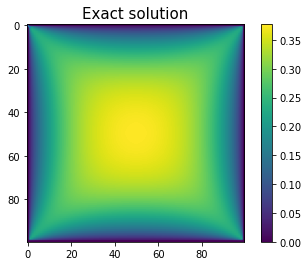
\includegraphics[width=0.5\textwidth]{./img/2d-paralelepipeds.png}
\caption{Plot of the Potential $\Phi$ for the 2-D square paralelepipeds}
\end{figure}


\section{Continuous Models}
We now want to move from discrete probability spaces and consider \emph{continuous} ones, where the base space $\Omega$ is uncountable.

A generalisation of the defintion of a P-space is given as follows

\begin{dfn}[]
  A (continuous) P-space is a tuple $(\Omega,\mathcal{A},\IP)$ if
  \begin{enumerate}
    \item $\mathcal{A}$ is a $\sigma$-Algebra.
    \item $\IP: \mathcal{A} \to [0,\infty]$ is $\sigma$-additive and normed ($\IP[\Omega] = 1$)
  \end{enumerate}
\end{dfn}
From measure theory, we know that we can extend $\mathcal{A}$ to the class of Lebesgue-measurable sets.

Although $\IP$ often cannot be extended to the complete powerset $\mathcal{P}(\Omega)$, that is often not necessary.

Instead of starting with the probabilty measure $\IP$ and analyze random variables as we did in the previous section, 
we can also go the other way around and introduce random variables $X_i$ and look for a $\IP$ that satisfies some properties with respect to the $X_i$.

For this, let's first consider the $0-1$ experiments, where
\begin{align*}
  \Omega = \{0,1\}^{\N} = \{\omega = (x_1,x_2,\ldots): x_i \in \{0,1\}\}
\end{align*}
and set $X_i(\omega) =x_i$ be the $i$-th component of the outcome.
Then, let $\mathcal{A}$ be the $\sigma$-Algebra generated by sets of the form $\{\omega: X_i(\omega) = 1\}, i = 1,2,\ldots$.
\begin{thm}[]
  Given a parameter $p \in [0,1]$, there exists a unique probability measure $\IP_p$ on $\mathcal{A}$ such that
  \begin{itemize}
    \item $\IP[X_i = 1] = p$ for all $i$
    \item The events $\{X_i = 1\}$ for all independent with respect to $\IP$.
  \end{itemize}
\end{thm}
\begin{proof}
It follows from the requirements on $\IP$ that for any choice of $x_1,\ldots,x_n$ we must have for $k = \sum_{i=1}^{n}x_i$
\begin{align*}
  \IP[X_1=x_1,\ldots,X_n=x_n] = \prod_{i=1}^{n}\IP[X_i=x_I]=p^{k}(1-p)^{n-k} 
\end{align*}
which automatically shows that $\IP$ is well defined on $\mathcal{A}$ and uniquely determins the events generated by finite union of the Form $\{X_1 = x_i, \ldots, X_n = x_n\}$.
By the Carathéodory-Hahn theorem from measure theory, such an extension exsists and is unique.
\end{proof}


\begin{lem}[Borel-Cantelli]
Let $A_1,\ldots,A_2, \ldots$ be a sequence of events in $\mathcal{A}$. And let
\begin{align*}
  A_{\infty} = \limsup_{n \to \infty}A_n = \bigcap_{n=1}^{\infty}\bigcup_{k=n}^{\infty}A_k
\end{align*}
be the set where infinitely many of the $A_k$ occur. Then
\begin{enumerate}
  \item $\sum_{k=1}^{\infty}\IP[A_k] < \infty$ implies $\IP[A_{\infty}] = 0$
  \item If the events $\left(A_{k}\right)_{k \in \N}$ are independent, then $\sum_{k=1}^{\infty}\IP[A_k] = \infty$ implies $\IP[A_{\infty}] = 1$.
\end{enumerate}
\end{lem}
\begin{proof}
  Since the sequence $B_n = \bigcup_{k \geq n}A_k$ is decreasing, 
The proof follows from the subadditivity that
\begin{align*}
  \IP[A_{\infty}] = \lim_{n \to \infty}\IP[B_n] \leq \lim_{n \to \infty}\sum_{k \geq n}\IP[A_k] = 0
\end{align*}
On the other hand, if they are independent, then we can write
\begin{align*}
  \IP\left[\bigcap_{k \geq n}A_k^{c}\right]
  =
  \prod_{k\geq n}\IP[A_k^{c}]
  =
  \prod_{k\geq n}(1 - \IP[A_k])
\end{align*}
and since the exponential function is convex, $1 - x \leq e^{-x}$, so \begin{align*}
  \IP\left[
\bigcap_{k \geq n}A_k^{c}
  \right]
  \leq
  \exp \left(
    - \sum_{k \geq n} \IP[A_k]
  \right)
   = 0
\end{align*}
and since the sequence $\bigcap_{k \geq n}A_k^{c}$ is increasing in $n$ it follows that
\begin{align*}
  \IP[A_{\infty}^{c}] = \lim_{n \to \infty} \IP\left[\bigcap_{k \geq n}A_k^{c}\right]= 0
\end{align*}
\end{proof}

Before proving (b), we first prove the next proposition
\begin{proposition}[]
	Let $R$ be a principal ideal domain and $p \in R$ irreducible. Then $(p)$ is a maximal ideal, and $p$ is prime.
\end{proposition}
Proof:	Let $J \subseteq R$ be an ideal such that $J \supsetneq (p)$. Since $R$ is a PID, there exists a $d \in R$ such that $J = (d) \supsetneq (p)$, which means that $d|p$, i.e. $\exists c \in R: p = dc$. Because $p$ is irreducible, we know that either $d$ or $c$ is a unit. If $c$ were a unit, we had $d = pc^{-1}$, but that would be that $d \in (p)$ which contradicts our assumption that $(d) \supsetneq (p)$. Therefore $d$ is a unit, which shows that $(d) = R$. In other words, $(p)$ is indeed a maximal ideal, and therefore $p$ is prime.\\

We also need one more proposition for the proof of the theorem
\begin{proposition}[]
	Let $R$ be a PID and let
	\begin{align*}
		J_0 \subseteq J_1 \subseteq J_2 \subseteq \ldots
	\end{align*}
	be an ascending chain of Ideals in $R$. Then there exists an $n \in \N$ such that $J_m = J_n$ for all $m \geq n$
\end{proposition}
Proof: Define $J = \bigcup_{n = \N} J_n$. Since it is the union of ideals containing the ideals lower in the chain, we know that $J$ itself is an ideal. And since $R$ is PID, $J = (d)$. But then there exists an $n \in N$ such that $J_n = (d) = J = J_m$ for $m \geq n$.\\


With this, we can easily prove (b) from the previous theorem:\\
Let $f \in R \setminus \{0\}$. If $f$ is a unit or is irreducible, then $f$ there is nothing to show.\\
Now assume that $f \in R \setminus \{0\}$ can not be written as a finite product of a unit and prime elements.
Assume that $f = f_0 = f_1 \tilde{f}_1$. If both $f_1$ or $\tilde{f}_1$ could be decomposed, then the same would be true for $f$. We may now assume that it is $f_1$ that can't be decomposed. Then we would ahve
\begin{align*}
	f_0 = f_1 \tilde{f}_1, f_1 = f_2 \tilde{f}_2, f_2 = f_3 \tilde{f}_3 \ldots
\end{align*}
In particular we would have a sequence of elements that divide each other: $f_{n+1} | f_n$ which means that we get an ascending chain of ideals
\begin{align*}
	(f_n) \subseteq (f_{n+1}), \quad \forall n \in \N
\end{align*}
Using the second proposition, we would have that there exists an $n \in \N$ such that $(f_{n}) = (f_{n+1})$. But since $R$ is a PID, we know that after looking at the prime elemnts which generate these ideals, that $f_{n} = a f_{n+1}$ for some unit $a \in R^{\times}$. And because the $\tilde{f}_n$ which contradicts the constructin of $f_n, \tilde{f}_n$.\\


For example, let's look at some prime numbers in $\Z[i]$. Some of them are $1 \pm i, 3, 2 \pm i$. Then we can describe the units of this Ring to be
\begin{align*}
	\Z[i]^{\times} = \{z \in \Z[i]\big\vert N(z) = 1\} = \{\pm 1, \pm i\}
\end{align*}
We also know that $2$ is not prime in $\Z[i]$ since $2 = (1+i)(1 -i)$ as well as $5 = (2+i)(2-i)$ is not prime either.


\begin{lemma}[]
	Let $z \in \Z[i]$ such that $N(z) = p \in \Z$ for $p$ prime in $\N$. Then $z$ is irreducible (and prime since $\Z[i]$ is a PID).
\end{lemma}
Proof: Let $z = uv$ for $u,v \in \Z[i]$. Then 
\begin{align*}
	p = N(z) = N(uv) = N(u)N(v) \implies \text{ wlog } N(u) = 1 \implies u \in \Z[i]^{\times}
\end{align*}

\begin{lemma}[]
	Let $p \in \N$ be prime in $\N$ that can not be written as a sum of two squares, then $p$ is also prime in $\Z[i]$
\end{lemma}
Proof: Assume $p = z \cdot w$. Then $N(z) \cdot N(w) = N(p) = p^2$. So $N(z) | p^2$ (in $\N$). So we have $N(z), N(w) \in \{1,p,p^2\}$. But we can remove $p$ from the list since
\begin{align*}
	N(z) = N(a + ib) = a^2 + b^2 = p \lightning
\end{align*}
contradicts the property of $p$, so wlog $N(z) = 1$ and $N(w) = p^2$. So one of them is a unit which shows that $p$ is irreducible (and prime).\\

In another example, we look at $K[X]$ for some field $K$. Then no polynomials of degree $0$ is irreducible, for they are the constants. If the degree is $1$, then every polynomial is irreducible. 
If the degree is $2$, then it is irreducible if and only if it has no zeros. If the degree is $3$, then we can use the same criterion as before. If the degree is $4$ however, we could have it as product of two polynomials of degree $2$ without zeros so the criterium doesn't work here.\\

In general, the question of finding irreducible polynomials depends alot on the field we are working with.\\


\subsection{Unique factorisation domain}

\begin{definition}[UFD]
	An integral domain $R$ is called a \textbf{unique factorisation domain} (or factorial ring) if every element $a \in R \setminus \{0\}$ can be written as a product of a unit and finitely many prime elements of $R$:
	\begin{align*}
		a = up_1 \dots p_n \quad \text{for} \quad u \in R^{\times}, p_1, \ldots p_n \text{ prim}
	\end{align*}
\end{definition}
Note: Every PID (and thus every euclidean Ring) is a UFD.
\begin{proposition}[]
	Let $R$ be a UFD. Then $p \in \setminus \{0\}$ is prime if and only if $p$ is irreducible.
\end{proposition}
Proof: As with any integral domain, prime implies irreducible. So let $p$ be irreducible. Because $R$ is a UFD, $p = u p_1 \dots p_n$, but since $p$ is irreducible, $n$ must be $1$, or else $p$ wouldn't be irreducible so $p = u p_1$. But becase $u$ is a unit, we have $(p) = (up_1) = (p_1)$ which means that $(p)$ is a prime ideal so $p$ is prime.\\


\begin{corollary}[]
	Let $R$ be an integral domain. Then $R$ is a UFD if and only if every element $a \in R \setminus \{0\}$ can be written as a product of a unit and finitely many irreducible elements and if the ring has the property that irreducible $\implies$ prime.
\end{corollary}

\begin{definition}[]
	Let $R$ be a commutative Ring and $a,b \in R$. We say $a$ and $b$ are \textbf{associated} and write $a \sim b$ if there exists a unit $u \in R^{\times}$ such that $a = ub$
\end{definition}

This also induces an equivalence relation. Reflexivity follows by chosing $u = 1$, symmetriy by using $b = u^{-1}a$ and transitivity comes from the product of the units $u_1$ and $u_2$.\\


\begin{lemma}[]
	Let $R$ be an integral domain and let $p,q$ be irreducible such that $p | q$. Then $p \sim q$
\end{lemma}
Proof: Becuase $p = ap$ and because $p$ is irreducible, and $q$ is not a unit, it follows that $a$ is a unit.\\

\begin{definition}[]
	For $n \in \N$ we define the \textbf{symmetric} group $S_n$ to be the set of consisting of the bijections
	\begin{align*}
		S_n := \left\{\sigma: \{1, \ldots, n\} \to \{1, \ldots, n\} \big\vert \sigma \text{ bijective}\right\}
	\end{align*}
\end{definition}
\begin{theorem}[Unique factorisation]
	Let $R$ be a unique factorisation domain. Then the factorisation of every nonzero element $a$ is unique up to permutation of the prime elements. In other words
	\begin{align*}
		up_1 \dots p_n = a = vq_1 \dots q_m \implies n = m \text{ and } \exists \sigma \in S_n: q_i \sim p_{\sigma(j)} \text{ for all } 1 \leq i \leq n
	\end{align*}
\end{theorem}

\begin{dfn}[]
Let $X$ be a $G$-space, $x \in X$. 
We call $G_x := \text{Stab}_G(x) = \{g \in G \big\vert gx = x\} \subseteq G$ the \textbf{stabilizer} of $x$.
\end{dfn}
Clearly, the stabilizer is a subgroup.

\begin{ex}[]
  Consider the group action of $SO(n)$ with the point $x = e_1 \in \mathbb{S}^{n-1}$.

  Its stabilizer $\text{Stab}_{SO(n)}(x)$ is isomorphic to $SO(n-1)$, as a matrix $A \in SO(n)$ satisfying $Ae_1 = e_1$ must be of the form
  \begin{align*}
    A = \begin{pmatrix}
    1 & 0\\
    0 & B
    \end{pmatrix}
    , \quad \text{where} \quad A^{T}A = 1 \implies B^{T}B = 1 \implies B \in SO(n-1)
  \end{align*}
  It is also a homoemorphism as $S^{n-1}$ is Hausdorff and $SO(n)/\text{Stab}_G(x)$ is compact (closed and bounded).
\end{ex}

A simple, yet powerful theorem is the \textbf{topological orbit theorem}.
\begin{thm}[Topological Orbit theorem]
Let $X$ be a $G$ space and $x \in X$.
Then the map
\begin{align*}
  F: \faktor{G}{\text{Stab}_{G}(x)} \to \mathcal{O}_G(x), \quad g \text{Stab}_G(x) \mapsto gx
\end{align*}
is a continuous bijection.
\end{thm}
\begin{proof}
  This mapping is indeed well defined, as
  \begin{align*}
    a \text{Stab}_G(x) = b \text{Stab}_G(x) \implies \exists h \in \text{Stab}_G(x) \text{ with } a = bh \implies ax = (bh)x = b(hx) = bx
  \end{align*}
  By definition of the orbit, it's clearly surjective.
  For injectivity, we have
  \begin{align*}
    ax = bx \implies a^{-1}(bx) = a^{-1}(ax) = x \implies a^{-1}b \in \text{Stab}_G(x)
  \end{align*}
  and for continuity, we see that the mapping
  \begin{align*}
    f \circ \pi: G \to \mathcal{O}x, \quad g \mapsto  gx
  \end{align*}
  is continuous and can use Lemma \ref{lem:unipropquot} to show continuity of $f$. 
\end{proof}


\subsection{Collapsing of subspaces to a point}
\begin{dfn}[]
Let $X$ be a topological space and $A \subseteq X$ a non-empty subset.
We write $X/A := X/\sim$ for 
\begin{align*}
  x \sim y \iff (x = y) \text{ or } x,y \in A
\end{align*}
\end{dfn}
We have already seen this type of spaces when discussing quotient topologies.
For example for $X = \mathbb{D}^{2}$ and $A = \del X = \mathbb{S}^{1}$, we got $X/A \iso \mathbb{S}^{2}$


\begin{dfn}[]
Let $X$ be a topolgical space and $A_{1}, \ldots, A_{n} \subseteq X$ be non-empty, pairwise disjoint subsets. 
We write $X/\left(
  A_{1}, \ldots, A_{n}
\right) := X/\sim$, where
\begin{align*}
  x \sim y \iff x = y \text{ or } \exists i: x,y \in A_i
\end{align*}
\end{dfn}
Note that if $X$ is metrizable (or $T_2,T_4$ ) and the $A_i$ are closed, then the quotient space is $T_2$. (We will prove this later when discussing $T_4$ spaces).

\begin{ex}[The cone]
  Given a topological space $X$, the quotient space 
  \begin{align*}
    \text{Cone}(X) :=
    \faktor{X \times [0,1]}{X \times \{1\}}
  \end{align*}
  is called the \textbf{cone} over $X$.
  The name becomes clear if we look at the case $X = \mathbb{S}^{1}$, in which case it resembles an (ice-cream) cone.
\end{ex}

\begin{ex}[Suspension]
  For a topological space $X$, the \textbf{suspension} of $X$ is the space
  \begin{align*}
    \Sigma(X) := \faktor{X \times [-1,1]}{X \times \{-1\}, X \times \{1\}}
  \end{align*}
  which can also be obtained by taking two cones and ``glueing'' them together at $X \times \{0\}$. 
  (What glueing is will be defined later but it should make intuitive sense).
\end{ex}

\begin{ex}[]
For a subset $A \subseteq X$ of a topological space, the \textbf{cone over $A$} is the space
\begin{align*}
  C_A(X) := \faktor{X \times [0,1]}{A \times \{1\}}
\end{align*}
\end{ex}

\begin{dfn}[Wedge \& Smash]
For $X, Y$ toplogical spaces with basepoints $x_0 \in X, y_0 \in Y$, we define
\begin{align*}
  \text{The \textbf{wedge} } X \vee Y &:= X \times \{y_0\} \cup \{x_0\} \times Y \subseteq X \times Y\\
  \text{The \textbf{smash} } X \wedge Y &:= \faktor{X \times Y}{X \vee Y}
\end{align*}
\end{dfn}

\begin{ex}[]
  For $X = \mathbb{S}^{n}$ and $Y = \mathbb{S}^{m}$ for $n,m \geq 1$ we have that $X \wedge Y = \mathbb{S}^{n+m}$.

To prove this, we see $\mathbb{S}^{n} = \R^{n} \cup \{\infty\}$ as the one-point-compactification of $\R^{n}$ and define the mapping \begin{align*}
  g: \R^{n} \cup \{\infty\} \times \R^{m} \cup \{\infty\} \to \R^{n+m} \cup \{\infty\}
\end{align*}
given by
\begin{align*}
  g(x,y) =
  \left\{\begin{array}{ll}
      (x,y)  & \text{ if } x \in \R^{n}, y \in \R^{m}\\
     \infty& \text{ otherwise}
  \end{array} \right.
\end{align*}
and showing that $g^{-1}(\infty) = X \vee Y$.
\end{ex}

\subsection{Glueing of topological spaces}
What glueing means intuitively should be clear, let's see if we can define it in a topological setting.

\begin{dfn}[]
Let $X,Y$ be topological spaces, $X_0 \subseteq X$ and $\phi: X_0 \to  Y$ continuous.
For the equivalence relation $\sim$ on $X \sqcup Y$ generated by $x \sim \phi(x)$, we write
\begin{align*}
  Y \cup_{\phi} X := \faktor{X \sqcup Y}{\sim}
\end{align*}
for the \textbf{glueing} of $X$ onto $Y$ by $\phi$.

\end{dfn}


\begin{rem}[]
  Note that the embedding $X \to Y \cup_{\phi}X, x \mapsto [x]$
  is continuous as it is equal to $\pi \circ \iota_X$, for $\iota_X$ the inclusion and $\pi$ the projection mapping.

  The glueing is a generalisation of the collapsing of subspaces, as for $A \subseteq X$, we have a homeomorphism
  \begin{align*}
    f: X/A \to \{\ast\} \cup_{\phi} X, \quad [x] \mapsto  [x]
  \end{align*}
  for $\phi: A \to \{\ast\}$, because $x,y \in A \iff \phi(x) = \phi(y)$.

    The mapping $Y \to Y \cup_{\phi} X, \quad y \mapsto [y]$ is also inective and a homeomorphism to its image as the map is not only continuous, but open.
    (The same might not be true for $X$)
\end{rem}

\begin{ex}[Mapping torus]
  Let $\alpha: X \to  X$ be a homeomorphism.
  We call
  \begin{align*}
    \faktor{X \times [0,1]}{\alpha} := \faktor{X \times [0,1]}{\sim}, \quad \text{ with } \quad (x,0) \sim (\alpha(x),1)
  \end{align*}
  the \textbf{mapping torus} of $\alpha$.
  
  \begin{itemize}
    \item The mapping torus of $\alpha = \id_{\mathbb{S}^{1}}$ is the ordinary \textbf{Torus}.
    \item The \textbf{Moebius strip} $M$ is the mapping torus of $\alpha: [-,1] \to  [-1,1], x \mapsto -x$.
    \item The \textbf{Klein bottle} $K$ is the mapping torus of $\alpha: \mathbb{S}^{1} \to \mathbb{S}^{-1}, z \mapsto \overline{z}$.
  \end{itemize}
  If we glue two Moebius strips together with the mapping 
  \begin{align*}
  \phi: 
  \underbrace{\pi(\{-1,1\} \times[0,1])}_{= \del M} \to M
  , \quad 
  m \to  m
  \end{align*}
  we obtain the Klein bottle $K = M \cup_{\phi} M$.
  To show this, we use the mapping
  \begin{align*}
    g: [-1,1] \times [0,1] \sqcup [-1,1] \times [0,1] \to  \mathbb{S}^{1} \times [0,1]
    \\
    (x,t) \cup (y,s) \mapsto (e^{i\pi x /2},t), (-e^{-i \pi y/2},s)
  \end{align*}

  
\end{ex}





Now, using our vector potential $\vec{\nabla} \times \vec{A} = \vec{B}$, we can re-write the maxwell equations to read
\begin{align*}
  \vec{E} = - \vec{\nabla}\Phi - \frac{\del \vec{A}}{\del t}
\end{align*}

The maxwell equations also imply charge conservation. 
Given that
\begin{align*}
 \epsilon_0c^{2} \vec{\nabla} \times \vec{B} 
 &= \vec{J} + \frac{\del \vec{E}}{\del t} \epsilon_0\\
 \implies
  0
 &=
 \vec{\nabla} \cdot \vec{J} + \frac{\del \rho}{\del t} = 0
\end{align*}
which when we integrate over the universe, we get
\begin{align*}
  0 
  &= \int_{\text{universe}} d^{3} \vec{x} \vec{\nabla} \cdot \vec{J} + \frac{\del }{\del t}\int_{\text{universe}} d^{3}\vec{x} \rho(\vec{x}
  \\
  &= \underbrace{\int_{\del \text{universe}} d \vec{S} \cdot \vec{J}}_{= 0} + \frac{\del Q_{\text{universe}}}{\del t} 
\end{align*}
where we say that there is no charge flowing ``out of the universe'' meaning twhich says that the total charge in the universe is constant.

Now, with the bac-cab identity for the curl of the curl,we can re-write
\begin{align*}
  c^{2} \vec{\nabla} \times \vec{B} 
  &= 
  \frac{\vec{J}}{\epsilon_0} + \frac{\del \vec{E}}{\del t}\\
  \implies
  c^{2} \left(
    \vec{\nabla}(\vec{\nabla \cdot \vec{A}}) - \nabla^{2} \vec{A}
  \right)
  &= \frac{\vec{J}}{\epsilon_0}
  +
  \frac{\del }{\del t}
  \left(
    - \vec{\nabla}\Phi - \frac{\del \vec{A}}{\del t}
  \right)
\end{align*}
which gives us the relation
\begin{align*}
  \left[\frac{1}{c^{2}}\frac{\del^{2}}{\del t^{2}} - \nabla^{2}\right] \vec{A}
  =
  \frac{\vec{J}}{\epsilon_0c^{2}} - \vec{\nabla} \left(
    \frac{1}{c^{2}} \frac{\del \Phi}{\del t} + \vec{\nabla}\vec{A}
  \right)
\end{align*}
which is not so nice as we simultanously need the scalar potential and the vector potential.
We will see later how we can only write it in terms of the vector potential.

Using our previous equation $\vec{E} = - \vec{\nabla} \Phi - \frac{\del \vec{A}}{\del t}$ and introducing the \textbf{d'Alembert Operator}
\begin{empheq}[box=\bluebase]{align*}
  \square := \frac{1}{c^{2}}\frac{\del^{2}}{\del t^{2}} - \nabla^{2}
\end{empheq}
we will later use symmetry to get
\begin{align*}
  \square \vec{A} = \frac{\vec{J}}{\epsilon_0c^{2}} \qquad
  \square \Phi = \frac{\rho}{\epsilon_0}
\end{align*}
\subsection{Gauge invariance}
The electric and magnetic field remain invariant under a simultanoues transformation known as \textbf{gauge transformation} given by
\begin{align*}
  \Phi \mapsto  \Phi' &= \Phi + \frac{\del }{\del t}f(\vec{x},t)\\
  \vec{A} \mapsto \vec{A}' &= \vec{A} - \nabla f(\vec{x},t)
\end{align*}
and after the substitution we get
\begin{align*}
  \square \Phi'  
  &= 
  \frac{\rho}{\epsilon_0} + \frac{\del }{\del t} \left(
    \frac{1}{c^{2}} \frac{\del \Phi'}{\del t} + \vec{\nabla} \cdot \vec{A}'
  \right)
  \square \vec{A}' = \frac{\vec{J}}{\epsilon_0 c^{2}} - \vec{\nabla} \left(
    \frac{1}{c^{2}} \frac{\del \Phi'}{\del t} + \vec{\nabla} \cdot \vec{A}
  \right)
\end{align*}
The idea then is that we choose $f(\vec{x},t)$ such that
\begin{align*}
  \frac{1}{c^{2}}\frac{\del \Phi'}{\del t} + \vec{\nabla} \cdot \vec{A}' = 0
\end{align*}
We will then find that the d'Alembert operator is consistent with the Lorentz transformation. So under the transformation
\begin{align*}
  \vec{x} \mapsto \vec{x}' &= \gamma(\vec{x} + \vec{v}t )\\
  t \mapsto t' &= \gamma(t - \frac{\vec{x} \cdot \vec{v}}{c^{2}}
\end{align*}
To find such an $f$, we first look for wave solutions
\begin{align*}
  f = f(\vec{n} \cdot \vec{x} + ct)
\end{align*}
then if we set $u := \vec{n} \cdot \vec{x} + ct$, we see
\begin{align*}
  \vec{\nabla}f = \frac{\del f(u)}{\del u}  \cdot \vec{n} \quad \text{and} \quad \frac{1}{c}\frac{\del f}{\del t} = \frac{\del f}{\del u} \cdot 1
\end{align*}
which means that its d'Alembert Operator evaluates to zero.
\begin{align*}
  \square f 
  = 
  \frac{1}{c^{2}} \frac{\del^{2}}{\del t^{2}}f - \nabla^{2}f 
  = 
  \frac{\del^{2}f}{\del u^{2}} - \frac{\del^{2}f}{\del u^{2}} \underbrace{u^{2}}_{=1} 
    = 0
\end{align*}
which is just saying that $f$ is indeed a wave.

If we write the electomagnetic fields as waves
\begin{align*}
  \vec{E} = \vec{e} f(\vec{n} \cdot \vec{x} + ct), \quad \vec{B} = \vec{b} f(\vec{n} \cdot \vec{x} + ct)
\end{align*}
then the maxwell equations show that they are perpendicular to each other, as
\begin{align*}
  0 = \vec{\nabla} \cdot \vec{E} = \hat{e_i}\hat{n}_i \del_u E = 0, \quad \vec{\nabla} \cdot \vec{B} = 0
\end{align*}
each imply that
\begin{align*}
 \vec{e} \cdot \vec{n} = 0 = \vec{b} \cdot \vec{n} 
\end{align*}
and by $\vec{\nabla} \times \vec{E} = - \frac{\del \vec{B}}{\del t}$ we get that
\begin{align*}
  \abs{\vec{E}} = c \abs{\vec{B}}
\end{align*}
The maxwell equations tell us that electromagnetic waves propagate at the speed of light.

Another example of wave functions are spherical waves.
There, we do not have have any angular dependence so
\begin{align*}
  \frac{1}{r} \frac{\del^{2}}{\del r^{2}}r + \underbrace{\frac{\vec{A}(\theta,\phi)}{r^{2}}}_{=0} = \nabla^{2}
\end{align*}
and if we assume then $\square f = 0$, we get
\begin{align*}
  \square f = \left[\frac{1}{c^{2}} \frac{\del^{2}}{\del t^{2}} - \frac{1}{r}\frac{\del^{2}}{\del r^{2}}r\right]f(r,t) = 0
\end{align*}
If we look for solutions of the form $f(r,t) = \frac{\psi(r,t)}{r}$ then the general solution is of the form
\begin{align*}
  \psi(r,t) = A(r + ct) + B(r - ct) \implies f(r,t) = \frac{A(r+ct) + B(r - ct)}{r}
\end{align*}
which we can interpret as ingoing and outgoing waves that decrease inamplitude as $r$ increases.

In many physical situations however is that we only have outgoing waves ($A = 0$).



\begin{cor}[]
  If $\gcd(p,n) = 1$, then $[\F_p[n]:\F_p]$ is a power of $p$ modulo $n$.
\end{cor}
To better understand what the group $\Z/n\Z^{\times}$ is like we show that we can decompose it into smaller copies, if $n$ is not a prime.

\begin{thm}[]
  If $\gcd(n,m) = 1$, then
  \begin{align*}
    (\Z/mn\Z)^{\times} \iso (\Z/m\Z)^{\times} \times (\Z/n\Z)^{\times}
  \end{align*}
  and if $p$ is prime $> 2$, then
  \begin{align*}
    (\Z/p^{r}\Z)^{\times} \iso \Z/p^{r-1} \times \Z/(p-1)\Z
  \end{align*}
  in particular, we have
  \begin{align*}
    (\Z,2^{r}\Z)^{\times} \iso \Z/2\Z \times (\Z/2^{r-2}\Z)
  \end{align*}
\end{thm}

For example we can calculate
$(\Z/7\Z)^{\times} = \{1,2,3,4,5,6\} \iso \Z/6\Z$
The possible exponents are $1,2,3,6$.
\begin{itemize}
  \item For $p = 2$, we have $2^{3} = 8 = 1 \mod 7$ and thus $[\F_p[7]:\F_2]= 3$ with 
    \begin{align*}
      \Phi_7(T) = (T^{3} + T + 1)(T^{3} + T^{2} + ) \in \F_[T]
    \end{align*}
  \item For $p = 3$, we need exponent $6$, and $\Phi_7$ is irreducible mod $3$.
  \item The prime $p = 13$, is of order $2$, because $13^{2} = 24 \cdot 7 + 1$. We then have
    \begin{align*}
      \Phi_7(T) = (T^{2} + 3T + 1)(T^{2} + 5T + 1)(T^{2} + 6T + 1)
    \end{align*}
  \item $p = 29$ is of order $1$ and
    \begin{align*}
      \Phi_7(T) = (T-7) (T-16)(T-20)(T-23)(T-24)(T-25)
    \end{align*}
\end{itemize}


\begin{thm}[]
  If $\gcd(p,n) = 1$, then the unitary irreducible factors of $\Phi_n$ if $\F_p[X]$ are all different and have the same degree of order $p \mod n$ in $(\Z(n\Z)^{\times}$.
\end{thm}

\begin{proof}
  Because $X^{n} -1$ has no multiple roots the same holds for $\Phi_n(X)$, therefore all irreducible factors have to be different.

  Since $\F_p[n]$, is a splitting field of $X^{n}-1$, we have that $\Phi_n(X)$ splits into linear factors in $\F_p[n][X]$, so the irreducible factors of $\Phi_n(X)$ must be of the FOrm $\text{irr}(\alpha,\F_p)$ for some $\alpha \in \F_p[n]$ with $\Phi_n(\alpha) = 0$.

  So it suffices to show that if $\Phi_n(\alpha) = 0$, then $\alpha$ must be a primitive $n$-th root of unity.
  From this, it would follow that $\F_p[n] = \F_p(\alpha)$ and the minimal polynomial $\text{irr}(\alpha,\F_p)$ has degree $[\F_p[n] : \F_p]$.

  Now assume that $\alpha$ is \emph{not} a primitive $n$-th root of unity with $\Phi_n(\alpha) = 0$.

  Then there exists a $1 \leq m <n$ with $\alpha^{m} = 1$ and suc that $m$ divides $n$.
  And we can write
  \begin{align*}
    0 = X^{m} - 1 = \prod_{l | m} \Phi_d(X) 
  \end{align*}
  so there has to be a $d_0 | m$ with $\Phi_{d_0}(\alpha) = 0$.
  But we can also write
  \begin{align*}
    X^{m} -1 = \Phi_n(X) \prod_{d|n, d < n} \Phi_d(X)
  \end{align*}
  so since $d_0$ divides $m$ and is a true divisor of $n$ we have that $\alpha$ must be a root of multiplicity at least two.
\end{proof}


Dirichlet proved that given some $a \in (\Z/n\Z)^{\times}$, there are finitely primes $p$ with $p = a \mod n$.


\begin{center}
Missing Second Half 28.05.21
\end{center}


\section{Appendix}
Solutions to old exams\footnote{We were the first year to have the algebra exam in written format. 
There are no old exams, so I just included the Mock Exam.} and exercise sheets from Algebra I \& II.

I obviously don't include all exercises, but those that I think are worth writing down.

\section*{Mock Exam FS 2021}


\subsection*{2.a}
Das Lemma über Fixpunkte sagt, dass für eine $p$-Gruppe $G$ und eine $G$-Menge $T$ gilt
$$
\abs{\text{Fix}_G(T)} \underset{\mod p}{=} \abs{T}.
$$
Wir betrachten die Gruppenwirkung 
$$
\rho: G \times G \to G, (g,h) \mapsto ghg^{-1}
$$
und sehen, dass 
$$
h \in \text{Fix}_G(G) \iff \forall g \in G: ghg^{-1} = h \iff h \in Z_G.
$$
Nach dem Lemma gilt also
$$
\abs{Z_G} =
\abs{\text{Fix}_G(G)} 
\underset{\mod p}{=} \abs{G} = p^{m} \underset{\mod p}{=} 0
$$
Nun ist das neutrale Element $1 \in G$ im Zentrum, also ist $\abs{Z_G}$ ein vielfaches von $p$ und darum nicht-trivial.

\subsection*{2.b}
Nach (a) hat $Z_G$ Ordnung $p^k$ für ein $1 \leq k \leq m$ und darum hat
$G^{(1)} := G/Z_G$ Ordnung $p^{m-k} < p^{m}$ und ist somit entweder trivial (und somit $G$ nilpotent), oder wiederum eine $p$-Gruppe.

Wiederholt man im zweiten Fall das Argument für $G^{(1)}$, so sieht man dass $G^{(2)} := G^{(1)}/Z_{G^{(1)}}$ wieder entweder trivial oder eine $p$-Gruppe ist und kleinere Ordnung als $G^{(1)}$ hat.

Macht man das für $G^{(k+1) := G^{(k)}/Z_{G^{(k)}}}$, falls $G^{(k)}$ nicht trivial, immer so weiter, so verkleinert sich die Ordnung.
  Da $G$ endlich ist, muss dieser Prozess aufhören, d.h. $\exists n \in \N: G^{(n)} = \{1\}$.
  Also ist $G$ nilpotent.


\subsection*{3}
  
Der Klassifikationssatz sagt folgendes aus:

Sei $R$ ein Hauptidealring und $M$ ein endlich erzeugtes Modul über $R$. 

Dann ist $M$ isomorph zu $R^n \times M_{\text{tors}}$, wobei $n$ der Rang von $M/M_{\text{tors}}$ ist.

Zum Beweis betrachten wir die Abbildung
$$
\Psi: R^{n} \times M_{\text{tors}} \to M
$$
$$
(a,m) \mapsto \sum_{i=1}^{n}a_i (x_i + M_{\text{tors}})
$$



\subsection*{4.a}
Für $\xi$ eine primitive $n$-te Wurzel von $1$ ist das $n$-te Zyklotomische Polynom definiert als
$$
\Phi_n(X) = \prod_{a \in A_n}(X - \xi^{a})
,
A_n = \{a \in \{1,\ldots,n-1\}\big\vert \ggT(a,n) = 1\}
$$
Wir zeigen 





\subsection*{7.a}
Sei $G$ eine Gruppe der Ordnung $8 = 2^{3}$.
Wir gehen alle Teiler von $8$ durch und schauen was passiert wenn $G$ Elemente solcher Ordnung enthält.

\begin{itemize}
  \item Enthält $G$ ein Element der Ordnung $8$, so ist $G \cong \mathbb{Z}/8 \mathbb{Z}$.
  \item Angenommen, ein Element $g\in G$ hat Ordnung $4$. 
    Für $N := \langle g\rangle$ ist $|G|/|H| = 2$ d.h. $N$ ist ein Normalteiler und $G/N \cong \mathbb{Z}/2 \mathbb{Z}$.

    Für ein $x \in G \setminus N$ gilt dann $x^{2}N = (xN)(xN) = N$, also $x^{2} \in N$.

    Weil $N$ durch $g$ generiert wird, wird $N$ auch von $xgx^{-1}$ generiert, da
    $$
    N = xNx^{-1} = \{1,xgx^{-1},xg^{2}x^{-1},xg^{3}x^{-1}\}
    $$
    des weiteren hat $xgx^{-1}$ auch Ordnung $4$ und ist darum entweder $xgx^{-1} = g$ oder $xgx^{-1} = g^{3}$.
    Wir wissen nun
    $$
    x^{2} \in \{1,g,g^{2},g^{3}\}, \text{ und } xgx^{-1} \in \{g, g^{3}\}
    $$
    (Man beachte dass nicht jede der $4 \cdot 2$ Möglichkeiten unbedingt alle Gruppenaxiome erfüllt z.B. $x^{2} = g, xgx^{-1} = g^{3}$ vertragen sich nicht. Wir betrachten nur die, die das tun.)
    \begin{itemize}
      \item Hat $x$ die Ordnung $8$, so ist $G \cong \mathbb{Z}/8 \mathbb{Z}$.
      \item Hat $x$ Ordnung $2$ und $xgx^{-1} = g$, so ist $G$ abelsch und $G \cong \mathbb{Z}/4 \mathbb{Z} \times \mathbb{Z}/2 \mathbb{Z}$.

        Ist $xgx^{-1} = g^{3}$, so beschreibt
        $$
        G = \langle x,g \big\vert x^{2} = 1, xgx^{-1} = g^{-1}\rangle
        $$
        gerade die Diedergruppe $D_{2 \cdot 4}$.

         \item Hat $x$ Ordnung $4$, so ist $x^{2} = g^{2}$.
           Im Falle $xgx^{-1} = g$ ist $G$ abelsch und
           $$(xg)^{2} = xgx^{-1} x^{2}g = gx^{2}g = g^{4} = 1
           $$
           d.h. $xg$ ist ein Element der Ordnung $2$ und somit $G \cong \mathbb{Z}/4 \mathbb{Z} \times \mathbb{Z}/2 \mathbb{Z}$.

           Im Fall $xgx^{-1} = g^{3}$, so beschreibt
           $$
           G = \langle x,g \big\vert g^{4} = 1, x^{2} = g^{2}, xgx^{-1} = g^{-1}\rangle
           $$
           die Quaternionengruppe $Q_8$.

    \end{itemize}

  \item Haben alle Elemente von $G$ Ordnung $\leq 2$, so ist $G \cong (\mathbb{Z}/2 \mathbb{Z})^{3}$.
\end{itemize}


\subsection*{7.b}
Sei $G$ eine abelsche Gruppe der Ordnung $50$.
Wir wissen vom Klassifikationssatz über endlich erzeugte abelsche Gruppen, dass 
$$
G \cong \mathbb{Z}/(d_1) \times \ldots \times \mathbb{Z}/(d_n)
$$
für $1 \leq d_1 | \ldots | d_n \neq 0$.
Die Grupppen sind also
$$
\mathbb{Z}/50 \mathbb{Z}, \quad \mathbb{Z}/5 \times \mathbb{Z}/10 \mathbb{Z}
$$


Alternativ betrachtet man die Primfaktorzerlegung $50 = 2 \cdot 5^{2} = 2 \cdot 5 \cdot 5$, und erhält
$$
\mathbb{Z}/2 \mathbb{Z} \times \mathbb{Z}/25 \mathbb{Z} \left(
  \cong \mathbb{Z}/50\mathbb{Z}
\right), \quad \mathbb{Z}/2 \mathbb{Z} \times \mathbb{Z}/5 \mathbb{Z} \times \mathbb{Z}/ 5 \mathbb{Z} \left(
  \cong \mathbb{Z}/10 \mathbb{Z} \times \mathbb{Z}/5 \mathbb{Z}
\right)
$$



\subsection*{8}
Angenommen $[K(\alpha) : K] = n$. Seien $g,h \in R[X]$ mit $f = gh$.






\subsection*{11}
Wir zeigen, dass $f := X^{4} - X - 1 \in \mathbb{Z}[X]$ irreduzibel und primitiv ist und wenden dann den Gauss'schen Satz an.

$f$ ist offensichtlich primitiv. Für Irreduzibilität verwenden wir folgende Proposition:
Sei $R$ ein faktorieller Ring, $p \in R$ prim, und $f \in R[X] \setminus \{0\}$.
Gilt für $f_{\mathrm{mod }p} \in R/(p)[X]$, dass $\mathrm{deg} f = \mathrm{deg} f_{\mathrm{mod }p}$ und $f_{\mathrm{mod }p} \in R/(p)[X]$ irreduzibel ist,
so ist $f \in R[X]$ prim.

Wir setzen $p=2$ und zeigen, dass $f_{\mathrm{mod }p} = X^{4} + X + 1 \in \mathbb{F}_2[X]$ irreduzibel ist.
Angenommen $f_{\mathrm{mod }p} = gh$ für $g,h \in \mathbb{F}_2[X]$. 
Dann ist o.B.d.A $\deg g \leq 2$.
Die irreduziblen Polynome in $\mathbb{F}_2[X]$ mit grad $\leq 2$ sind gerade
$$
X, X + 1, X^{2} + X + 1
$$
Den Faktor $x$ ist offensichtlich nicht möglich und
den Fall $\deg g = \deg h = 2$ können wir ausschliessen, da $(X^{2} + X + 1)^{2} = X^{4} + X^{2} + 1 \neq f_{\mathrm{mod }p}$.

Des weiteren ist ein Polynom genau dann durch $X+1$ teilbar, wenn die Summe der Koeffizienten gerade ist. 
Das ist bei $f_{\mathrm{mod }p}$ nicht der Fall, also ist $f_{\mathrm{mod }p}$ irreduzibel in $\mathbb{F}_2[X]$.

Nach der Proposition ist $X^{4} - X - 1 \in \mathbb{Z}[X]$ irreduzibel und nach dem Gauss'schen Satz auch in $\mathbb{Q}[X]$.

\subsection*{12}
Nach dem Eisenstein Kriterium für $p = 5$ ist $f := X^{5} - 20 X + 5 \in \mathbb{Q}[X]$ irreduzibel.

Des weiteren ist 
$$f' = 5X^{4} - 20X = 5(X^{4} - 4)$$
mit $2$ reellen Nullstellen $\pm \sqrt[4]{4} = \pm \sqrt{2}$.
$f$ hat also $3 = p-2$ reelle Nullstellen und nach Satz \ref{thm:p-minus-two-roots} ist $\Gal(f) \cong S_5$.







\section{Scratchpad}
Unordered collection of explanations and results from outside the lectures.
Some content is from the exercise classes.

Given a field extension $L/k$ and $\alpha \in E$, consider the evaluation mapping
\begin{align*}
  \ev_{\alpha}: k[X] \to L, \quad f \mapsto f(\alpha)
\end{align*}

\begin{itemize}
  \item If $\alpha$ is a root of some non-constant polynomial $f \in k[X]$, we say that $\alpha$ is \textbf{algebraic} over $k$.
    If that is the case, then $\Ker \ev_{\alpha} = (m_{\alpha})$ is a principal (and thus maximal) ideal for some $\mu_{\alpha} \in k[X]$ called the \textbf{minimal polynomial} of $\alpha$.
    As $k[X]/(m_{\alpha})$ is already a field, the smallest field containing $\alpha$ is
    \begin{align*}
      k(\alpha) = \Image \ev_{\alpha} \iso \faktor{k[X]}{(m_{\alpha})}
    \end{align*}
  \item If the evaluation mapping is injective, we say that $\alpha$ is \textbf{transcendental}.
    Therefore $k[\alpha] \iso k[X]$, and the smallest field containing $\alpha$ is
    \begin{align*}
      k(\alpha) = \text{Quot}(k[\alpha]) \iso \text{Quot}(k[X]) = k(X) = \{\frac{f}{g} \big\vert f,g \in k[X], g \neq 0\}
    \end{align*}
\end{itemize}

The notation $k[\alpha]$ for $\Image \ev_{\alpha}$ coincides with the notation we use when writing $\Q[i]$.
Moreover, if we think of the ``free variable'' $X$ as a ``foreign'' transcendental number living in some extension, we recover the definition of the polynomial ring $k[X]$



\begin{ex}[]

Say we know some $\alpha \in \C$ has minimal polynomial $X^{4} - X - 1 \in \Q[X]$.
From our above consideration, we know that $k(\alpha) = \Image \ev_{\alpha}$.
Now if we want to understand what $\Image \ev_{\alpha}$ actually looks like, we plug in $\alpha$ into all polynomials $f \in k[X]$ to get numbers of the form
\begin{align*}
  f(\alpha) = \sum_{k=0}^{n} a_k\alpha^{k} \in \C
\end{align*}
and identify them using the minimal polynomial, which tells us that $\alpha^{4} - \alpha - 1 = 0$, or in other words: $\alpha^{4} = 1 + \alpha$.
This tells us that anytime the exponent of $\alpha$ is $\geq 4$, we can reduce it. 
For example, the number $\alpha^{6}$ can be re-written as
\begin{align*}
  \alpha^{6} = \alpha^{2} \alpha^{4} = \alpha^{2} (1 + \alpha) = \alpha^{2} + \alpha^{3}
\end{align*}
It's easy to see that then $1,\alpha,\alpha^{2},\alpha^{3}$ form a basis of $\Q(\alpha)$.
To make sure that numbers of the form
\begin{align*}
  a_0 + a_1 \alpha + a_2 \alpha^{2} + a_3 \alpha^{3}
\end{align*}
form a field with the induced multiplication, let's compute the inverse of $\alpha$ and $\alpha+1$.

The inverse of $\alpha$ should satisfy $\alpha^{-1} \alpha = 1$.
And another way of writing $1$ is $1 + 0 = 1 + \alpha^{4} - \alpha - 1 = \alpha^{4} - \alpha$. Giving us
\begin{align*}
  \alpha^{-1} \alpha = 1 = \alpha^{4} - \alpha \implies \alpha^{-1} = \alpha^{3} - 1
\end{align*}
For $\alpha + 1$, we know that $\alpha^{4} = \alpha + 1$, so
\begin{align*}
  (\alpha +1)^{-1} = (\alpha^{4})^{-1} = (\alpha^{-1})^{4} = (\alpha^{3} - 1)^{4}
\end{align*}
The term on the right will contain some $\geq 4$ order terms, but as mentioned earlier, they can easily be reduced.
\end{ex}





\section{Useful theorems, propositions, results}

\subsection{Rings}
\begin{table}[h]
\centering
\begin{tabular}{L|L|L|L|L|L|L}
  \text{Fields} 
  & \text{Euclidean Ring} 
  & \text{PID} 
  & \text{UFD} 
  & \text{Integral Domain} 
  & \text{Commutative} 
  & \text{Ring}\\ \hline
  %%%%
  \Q,\R,\C
  & \Z, K[X], \Z[i]
  & \Z[ \frac{1 + i \sqrt{19}}{2}]
  & \Z[X,Y]
  & \Z[i \sqrt{5}]
  & C([0,1])
  & \Mat_{n \times n}(R)\\
  %%%%
  \Z/p\Z
  & \Z[i \sqrt{2}], \Z[\sqrt{3}] 
  &
  & K[X_1,\ldots,X_n]
  &
  & \Z/n\Z
  \\
  %%%%
  & 
  & 
  & \text{prime $\iff$ irred.}
\end{tabular}
\caption{Example of rings. The inclusion goes from left to right.}
\end{table}

\subsection{Polynomial Rings}
\begin{itemize}
  \item $f = a_0 + \ldots a_nX^{N}\in R[X]^{\times}$ if and only if $a_0 \in R^{\times}$ and each $a_i, i > 0$ is a zero divisor.
\end{itemize}



\subsection{Field extensions}

\subsection{Separability}
\begin{itemize}
  \item If $f \in k[X]$ is separable, then for any extension $L/k$, $f\in E[X]$ is also separable.
  \item If $E$ is a splitting field of a separable and irreducible polynomial $f \in k[X]$ then $\degree f$ divides $\abs{\Gal(E/k)}$.
    Proof: For a root $\alpha$: $\abs{\Gal(E/k)} = [E:k] = [E:k(\alpha)] [k(\alpha):k]$.
  \item Let $f \in k[X]$ is irreducible. If either $\charac k = 0$ or $\degree f' = \degree f-1$, then $f$ is separable.
\end{itemize}




\subsection{Galois Theory}
Let $E/k$ be a field extension. TFAE:
\begin{itemize}
  \item $E/k$ is Galois.
  \item $E^{\Gal(E/k)} = k$
  \item $\abs{\Gal(E/k)} = [E:k]$.
\end{itemize}

%\subsection{Computing the Galois group}
%Usually, when computing the Galois group, we apply many tricks to find out more and more information about the group until we can uniquely determine it.
%
%Some tricks tell us how the galois group can 
%
%\begin{itemize}
%  \item If $f$ is a separable polynomial with $n$ roots, we know that the Galoisgroup is a subgroup of $S_n$.
%
%\end{itemize}


\end{document}

